%%%%%%%%%%%%%%%%%%%%%%%%%%%%%%%%%%% SETUP
\documentclass{classes/beamer_GeomaticaUA}
%\documentclass[handout]{Classes/beamer_GeomaticaUA}
\usepackage{styles/beamer_GeomaticaUA}
%\usepackage{styles/Amsterdam}
\usepackage{listings}
\renewcommand{\lstlistlistingname}{Codes}
\renewcommand{\lstlistingname}{Code}


%% LISTING ENVIRONMENTS-----------------------
% Java/c#
\lstnewenvironment{Java}{\lstset{
language=Java,                % choose the language of the code
 frame=Ltbr,
 framerule=0.2pt,
 aboveskip=0.5cm,
 framextopmargin=3pt,
 framexbottommargin=3pt,
 framexleftmargin=0.4cm,
 framesep=0.4pt,
 rulesep=0.4pt,
 %backgroundcolor=\color{white},
 rulesepcolor=\color{gray},
 stringstyle=\ttfamily\color{purple},
 showstringspaces = false,
 %basicstyle=\small\ttfamily,
 commentstyle=\color[rgb]{0.133,0.545,0.133},
 keywordstyle=\color[rgb]{0,0,1},%\bfseries 
 %morekeywords={text,serial,with,owner,to, replace, function, for, if, begin, loop, exit,
 %return,returns,cost,row,volatile,into, setof, double, precision,declare,record,reverse,boolean},
 numbers=left,
 numbersep=14pt,
 breaklines=true
}}{}

% SQL
\lstnewenvironment{SQL}{\lstset{
language=SQL,                % choose the language of the code
 frame=Ltbr,
 framerule=0.2pt,
 aboveskip=0.25cm,
 framextopmargin=3pt,
 framexbottommargin=3pt,
 framexleftmargin=0.4cm,
 framesep=0.4pt,
 rulesep=0.4pt,
 backgroundcolor=\color{white},
 rulesepcolor=\color{gray},
 stringstyle=\ttfamily\color{purple},
 showstringspaces = false,
 basicstyle=\tiny\ttfamily,
 commentstyle=\color[rgb]{0.133,0.545,0.133},
 keywordstyle=\color[rgb]{0,0,1},%\bfseries 
 morekeywords={text,serial,with,owner,to, replace, function, for, if, begin, loop, exit,
 return,returns,cost,row,volatile,into, setof, double, precision,declare,record,reverse,boolean},
 numbers=left,
 numbersep=14pt,
 breaklines=true,
 extendedchars=true,
 literate={á}{{\'a}}1 {é}{{\'e}}1 {í}{{\'i}}1 {ó}{{\'o}}1 {ú}{{\'u}}1 {ñ}{{\~n}}1 {¿}{{?`}}1
}}{}


% Defino un entorno CommandLine Linux
\lstnewenvironment{bash}{\lstset{
language=bash,                % choose the language of the code
 frame=Ltbr,
 framerule=0.2pt,
 aboveskip=0.25cm,
 framextopmargin=3pt,
 framexbottommargin=3pt,
 framexleftmargin=0.4cm,
 framesep=0.4pt,
 rulesep=0.4pt,
 backgroundcolor=\color{white},
 rulesepcolor=\color{gray},
 stringstyle=\ttfamily\color{purple},
 showstringspaces = false,
 basicstyle=\tiny\ttfamily,
 commentstyle=\color[rgb]{0.133,0.545,0.133},
 keywordstyle=\color[rgb]{0,0,1},%\bfseries
 morekeywords={cd,mkdir}
 numbers=left,
 numbersep=14pt,
 breaklines=true,
 extendedchars=true,
 literate={á}{{\'a}}1 {é}{{\'e}}1 {í}{{\'i}}1 {ó}{{\'o}}1 {ú}{{\'u}}1 {ñ}{{\~n}}1 {¿}{{?`}}1
}}{}


% PLR
\lstnewenvironment{PLR}{\lstset{
language=R,                % choose the language of the code
 frame=Ltbr,
 framerule=0.2pt,
 aboveskip=0.5cm,
 framextopmargin=3pt,
 framexbottommargin=3pt,
 framexleftmargin=0.4cm,
 framesep=0.4pt,
 rulesep=0.4pt,
 %backgroundcolor=\color{white},
 rulesepcolor=\color{gray},
 stringstyle=\ttfamily\color{purple},
 showstringspaces = false,
 %basicstyle=\small\ttfamily,
 commentstyle=\color[rgb]{0.133,0.545,0.133},
 keywordstyle=\color[rgb]{0,0,1},%\bfseries 
 morekeywords={text,serial,with,owner,to, replace, function, for, if, begin, loop, exit,
 return,returns,cost,row,volatile,into, setof, double, precision,declare,record,reverse},
 numbers=left,
 numbersep=14pt,
 breaklines=true
}}{}

% R
\lstnewenvironment{R}{\lstset{
language=R,                % choose the language of the code
 frame=Ltbr,
 framerule=0.2pt,
 aboveskip=0.5cm,
 framextopmargin=3pt,
 framexbottommargin=3pt,
 framexleftmargin=0.4cm,
 framesep=0.4pt,
 rulesep=0.4pt,
 %backgroundcolor=\color{white},
 rulesepcolor=\color{gray},
 stringstyle=\ttfamily\color{purple},
 showstringspaces = false,
 alsoother={:_\$},
 %basicstyle=\small\ttfamily,
 commentstyle=\color[rgb]{0.133,0.545,0.133},
 keywordstyle=\color[rgb]{0,0,1},%\bfseries 
 %morekeywords={text,serial,with,owner,to, replace, function, for, if, begin, loop, exit,
 %return,returns,cost,row,volatile,into, setof, double, precision,declare,record,reverse},
 numbers=left,
 numbersep=14pt,
 breaklines=true
}}{}

% PHP
\lstnewenvironment{PHP}{\lstset{
language=PHP,                % choose the language of the code
 frame=Ltbr,
 framerule=0.2pt,
 aboveskip=0.5cm,
 framextopmargin=3pt,
 framexbottommargin=3pt,
 framexleftmargin=0.4cm,
 framesep=0.4pt,
 rulesep=0.4pt,
 %backgroundcolor=\color{white},
 rulesepcolor=\color{gray},
 stringstyle=\ttfamily\color{purple},
 showstringspaces = false,
 %basicstyle=\small\ttfamily,
 commentstyle=\color[rgb]{0.133,0.545,0.133},
 keywordstyle=\color[rgb]{0,0,1},%\bfseries 
 numbers=left,
 numbersep=14pt,
 breaklines=true
}}{}

% Diagramas entidad relación
% Ver ejemplo en http://heisenbugs.blogspot.com.es/2010/10/making-great-er-diagrams-without.html
\usepackage{styles/tikz-er2}
\usetikzlibrary{positioning}
\usetikzlibrary{shadows}
\usetikzlibrary{mindmap}
% Diagramas UML
% Ver http://perso.ensta-paristech.fr/~kielbasi/tikzuml/index.php?lang=en
\usepackage{styles/tikz-uml}

%% ER styles
\tikzstyle{every entity} = [top color=white, bottom color=blue!30,
draw=blue!50!black!100, drop shadow]
\tikzstyle{every weak entity} = [drop shadow={shadow xshift=.7ex,
shadow yshift=-.7ex}]
\tikzstyle{every attribute} = [top color=white, bottom color=yellow!20,
draw=yellow, node distance=7em, drop shadow]
\tikzstyle{every relationship} = [top color=white, bottom color=red!20,
draw=red!50!black!100, drop shadow]
\tikzstyle{every isa} = [top color=white, bottom color=green!20,
draw=green!50!black!100, drop shadow]


%% Árboles de directorios
%\usepackage{tikz}
%\usetikzlibrary{trees}

%\tikzstyle{every node}=[draw=black,thick,anchor=west]
%\tikzstyle{selected}=[draw=red,fill=red!30]
%\tikzstyle{optional}=[dashed,fill=gray!50]

%%%%%%%%%%%%%%%%%%%%%%%%%%%%%%%%%%%
%\begin{frame}{Modelo Jerárquico}
%\begin{columns}
%\begin{column}{0.5\textwidth}
%\begin{center}

%\begin{tikzpicture}[%
%  grow via three points={one child at (0.5,-0.7) and
%  two children at (0.5,-0.7) and (0.5,-1.4)},
%  edge from parent path={(\tikzparentnode.south) |- (\tikzchildnode.west)}]
%  \node {País}
%    child { node {Prov A}}		
%    child { node [selected] {Prov C}
%      child { node {Muni C1}}
%      child { node [selected]{Muni C2}
%      	child { node [selected] {Parc 1}}
%      	child { node [selected] {Parc2}}
%      	child { node [selected] {Parc n}}
%      }
%      child [missing] {}	
%      child [missing] {}				
%	  child [missing] {}	
%      child { node [optional] {Muni C$n$}}
%    }
%    child [missing] {}				
%    child [missing] {}	
%    child [missing] {}				
%    child [missing] {}	
%    child [missing] {}							
%    child [missing] {}				
%    child { node [optional] {Prov $n$}};
%\end{tikzpicture}
%\end{center}
%\end{column}
%
%\begin{column}{0.5\textwidth}
%El modelo jerárquico organiza los datos en una estructura ramificada (\textit{tree structure}).\\[3ex]
%
%\textbf{Consulta:}\\
%Cultivos/superficie en el municipio C2\\[3ex]
%
%\textbf{Coste:} \\
%Una búsqueda por Prov, otra por Muni de la Prov C y calculamos las estadísticas para todos. No hay que seguir buscando.
%\end{column}
%\end{columns}
%\end{frame}

%%%%%%%%%%%%%%%%%%%%%%%%%%%%%%%%%%% METADATA
\author{Miguel Fernández Moreno}
\title{PostGIS (II)}
\titlegraphic{
\includegraphics[height=0.6cm]{logos/logo_ua.png} \hspace{1cm} 
\includegraphics[height=1cm]{logos/iig}} 
\institute[GeomaticaLab]{Instituto Interuniversitario de Geografía\\Laboratorio de Geomática} 
\date{13 de noviembre de 2014}
\subject{Cuarta sesión del curso ``Diseño, creación y gestión de Bases de Datos Geográficas con PostGIS''}


%%%%%%%%%%%%%%%%%%%%%%%%%%%%%%%%%%% SLIDES
\begin{document}

\begin{frame}
\titlepage
\end{frame}

\section[Introducción]{Presentación y comentarios}
\subsection{Descripción general del SQL}
%%%%%%%%%%%%%%%%%%%%%%%%%%%%%%%%%%%
\begin{frame}{¿Que vamos a hacer hoy?}
\begin{enumerate}
\item Índices espaciales
\item Operadores espaciales
\item Geoprocesamiento
\end{enumerate}
\end{frame}


\section[Índices]{Índices espaciales}
%%%%%%%%%%%%%%%%%%%%%%%%%%%%%%%%%%%
\begin{frame}[fragile]
\frametitle{El índice en una base de datos}
Estructura de datos que mejora la velocidad de las operaciones, por medio de un identificador único de cada fila de una tabla, permitiendo un rápido acceso a los registros de una tabla en una base de datos. 
\end{frame}

\begin{frame}[fragile]
\frametitle{¿Por qué usarlos?}
\begin{itemize}
\item Evitamos un lectura completa de la tabla
\item Rápidez en la ejecución de las consultas
\item Evitamos sobrecarga de CPU, sobrecarga de disco y concurrencia
\item Es una ventaja en tablas con gran cantidad de datos
\end{itemize}
\end{frame}

% --------------------------------------------------- Slide --
\begin{frame}[fragile]
\frametitle{Índices PostgreSQL / Postgis}
\begin{description}
\item[B-Trees]\hfill \\ Se usa para datos que pueden ser ordenados sobre un eje: números, letras, fechas. No es aplicable a los datos GIS.
\item[R-Trees] \hfill \\Divide los datos en rectángulos, sub-rectángulos, sub-sub-rectángulos, etc.
\item[GiST] \hfill \\Parte los datos \emph{cosas que están a un lado}, \emph{cosas que se superponen}, \emph{cosas que están dentro}. PostGIS utiliza un índice R-Tree implementado en la parte superior de GiST para indexar los datos GIS.
\end{description}
\end{frame}
% --------------------------------------------------- Slide --
\begin{frame}[fragile]
\frametitle{Crear índice usando GiST}
\lstset{caption=Ejemplo de índice GiST,label=sql:gist}
\begin{SQL}
-- La sintaxis para crear un índice GiST en la columna geometría:
CREATE INDEX index_ua_pc2 ON ua_pc2 USING GIST (geom);
\end{SQL}

\end{frame}
% --------------------------------------------------- Slide --
\begin{frame}[fragile]
\frametitle{GiST}
\lstset{caption=Comprobar velocidad del índice GiST,label=sql:qIndex}
\begin{SQL}
-- Sintaxis para comprobar el funcionamiento del índice:
SELECT codigo ,avg(z) AS media FROM estancias, ua_pc2
WHERE st_intersects(estancias.geom, ua_pc2.geom) 
GROUP BY codigo;
\end{SQL}

\end{frame}
% --------------------------------------------------- Slide --
\begin{frame}[fragile]
\frametitle{Funcionamiento de la consulta con el índice}
\begin{block}{Resultado sin índice}
\center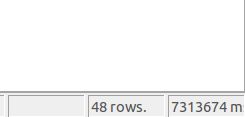
\includegraphics[scale=0.5]{images/resultWithoutIndex.png}
\end{block}
\begin{block}{Resultado con índice}
\center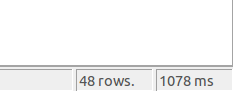
\includegraphics[scale=0.5]{images/resultWithIndex.png}
\end{block}
\end{frame}
% --------------------------------------------------- Slide --
\begin{frame}[fragile]
\frametitle{Funcionamiento de la consulta con el índice}
\center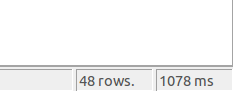
\includegraphics[scale=0.5]{images/resultWithIndex.png}
\end{frame}
% --------------------------------------------------- Slide --
\section[Operadores]{Operadores espaciales}
%%%%%%%%%%%%%%%%%%%%%%%%%%%%%%%%%%%
\begin{frame}[fragile]
\frametitle{Operadores espaciales (I)}
\begin{description}
\item[\&\&]Devuelve TRUE si la bounding box de la geometría A intersecta con la bounding box de la geometría B.
\item[\&$<$]Devuelve TRUE si la bounding box de A solapa o está a la izquierda de B.
\item[\&$<|$]Devuelve TRUE si la bounding box de A solapa o está bajo de B.
\item[\&$>$]Devuelve TRUE si la bounding box de A solapa o está a la derecha de B.
\item[$<<$]Devuelve TRUE si la bounding box de A está estrictamente a la izquierda de B.
\item[$<<|$]Devuelve TRUE si la bounding box de A está estrictamente bajo de B.
\end{description}
\end{frame}
% --------------------------------------------------- Slide --
\begin{frame}[fragile]
\frametitle{Operadores espaciales (II)}
\begin{description}
\item[=]Devuelve TRUE si la bounding box de A es la misma que la de B. Usa doble precisión.
\item[$>>$]Devuelve TRUE si la bounding box de A es estrictamente a la derecha de B.
\item[$@$]Devuelve TRUE si la bounding box de A está contenida por la de B.
\item[$\mid$\&$>$]Devuelve TRUE si la bounding box de A solapa o está arriba de la de B.
\item[$\mid\gg$]Devuelve TRUE si la bounding box de A está estrictamente arriba de la de B.
\item[$\thicksim$]Devuelve TRUE si la bounding box de A contiene la de B.
\end{description}
\end{frame}
% --------------------------------------------------- Slide --
\begin{frame}[fragile]
\frametitle{Operadores espaciales (III)}
\begin{description}
\item[$~=$]Devuelve TRUE si la bounding box de A es la misma que la de B.
\item[$<->$]Devuelve la distancia entre dos puntos. F
\item[$<\#>$]Devuelve la distancia entre la bounding box de dos geometrías. 
\end{description}
\end{frame}

\section[Ejercicios]{Operadores espaciales}
%%%%%%%%%%%%%%%%%%%%%%%%%%%%%%%%%%%
% --------------------------------------------------- Slide --

% --------------------------------------------------- Slide --

\section[Geoprocesamiento]{Geoprocesamiento}
%%%%%%%%%%%%%%%%%%%%%%%%%%%%%%%%%%%
% --------------------------------------------------- Slide --
\begin{frame}[fragile]
\frametitle{Geoprocesamiento (I)}
\begin{description}
\item[st\_buffer] (T) For geometry: Returns a geometry that represents all points whose distance from this Geometry is less than or equal to distance. Calculations are in the Spatial Reference System of this Geometry. For geography: Uses a planar transform wrapper.
\item[st\_buildArea] — Creates an areal geometry formed by the constituent linework of given geometry
\item[st\_collect] — Return a specified ST\_Geometry value from a collection of other geometries.
\item[st\_concaveHull] — The concave hull of a geometry represents a possibly concave geometry that encloses all geometries within the set. You can think of it as shrink wrapping.
\end{description}
\end{frame}
% --------------------------------------------------- Slide --

\begin{frame}[fragile]
\frametitle{Geoprocesamiento (II)}
\begin{description}
\item[st\_convexHull] — The convex hull of a geometry represents the minimum convex geometry that encloses all geometries within the set.
\item[st\_curveToLine] — Converts a CIRCULARSTRING/CURVEDPOLYGON to a LINESTRING/POLYGON
\item[st\_delaunayTriangles] — Return a Delaunay triangulation around the given input points.
\item[st\_difference] — Returns a geometry that represents that part of geometry A that does not intersect with geometry B.
\item[ST\_Dump] — Returns a set of geometry\_dump (geom,path) rows, that make up a geometry g1.
\item[ST\_DumpPoints] — Returns a set of geometry\_dump (geom,path) rows of all points that make up a geometry.
\item[ST\_DumpRings] — Returns a set of geometry\_dump rows, representing the exterior and interior rings of a polygon.
\end{description}
\end{frame}
% --------------------------------------------------- Slide --

\begin{frame}[fragile]
\frametitle{Geoprocesamiento (III)}
\begin{description}
\item[ST\_FlipCoordinates] — Returns a version of the given geometry with X and Y axis flipped. Useful for people who have built latitude/longitude features and need to fix them.
\item[ST\_Intersection] — (T) Returns a geometry that represents the shared portion of geomA and geomB. The geography implementation does a transform to geometry to do the intersection and then transform back to WGS84.
\item[ST\_LineToCurve ]— Converts a LINESTRING/POLYGON to a CIRCULARSTRING, CURVED POLYGON
\item[ST\_MakeValid] — Attempts to make an invalid geometry valid without losing vertices.
\item[ST\_MemUnion] — Same as ST\_Union, only memory-friendly (uses less memory and more processor time).
\item[ST\_MinimumBoundingCircle] — Returns the smallest circle polygon that can fully contain a geometry. Default uses 48 segments per quarter circle.
\item[ST\_Polygonize] — Aggregate. Creates a GeometryCollection containing possible polygons formed from the constituent linework of a set of geometries.

\end{description}
\end{frame}

\begin{frame}[fragile]
\frametitle{Geoprocesamiento (IV)}
\begin{description}
\item[ST\_Node] — Node a set of linestrings.
\item[ST\_OffsetCurve] — Return an offset line at a given distance and side from an input line. Useful for computing parallel lines about a center line
\item[ST\_RemoveRepeatedPoints] — Returns a version of the given geometry with duplicated points removed.
\item[ST\_SharedPaths] — Returns a collection containing paths shared by the two input linestrings/multilinestrings.
\item[ST\_Shift\_Longitude] — Reads every point/vertex in every component of every feature in a geometry, and if the longitude coordinate is <0, adds 360 to it. The result would be a 0-360 version of the data to be plotted in a 180 centric map
\item[ST\_Simplify] — Returns a "simplified" version of the given geometry using the Douglas-Peucker algorithm.
\item[ST\_SimplifyPreserveTopology] — Returns a "simplified" version of the given geometry using the Douglas-Peucker algorithm. Will avoid creating derived geometries (polygons in particular) that are invalid.
\item[ST\_Split] — Returns a collection of geometries resulting by splitting a geometry.
\item[ST\_SymDifference] — Returns a geometry that represents the portions of A and B that do not intersect. It is called a symmetric difference because ST\_SymDifference(A,B) = ST\_SymDifference(B,A).
\item[ST\_Union] — Returns a geometry that represents the point set union of the Geometries.
\item[ST\_UnaryUnion] — Like ST\_Union, but working at the geometry component level.
\end{description}
\end{frame}


% --------------------------------------------------- Slide --
\end{document}
